\documentclass[runningheads]{llncs}
\usepackage{amsmath,amssymb,amstext}
\usepackage{bm}
\usepackage{CJK}
\usepackage{graphicx}
\usepackage{subfigure}
\usepackage{tikz}
\usetikzlibrary{fit,positioning}

\begin{document}
\title{Explainable Functional Region Identification}
\author{Submission}

\maketitle

\begin{abstract}
As a critical step in urban computing, functional region identification (FRI) has attracted a lot of research attention.
Existing research generally cluster city regions based on human mobility data where the cluster labels are difficult to interpret.
In this paper, we explore the problem of explainable functional region identification (EFRI), which integrates online geo-tagged textual data and mobility data to deliver explanations of any FRI results.
We  explain a region's function through a set of urban activities and urban features, which are automatically extracted from online textual data.
We  build a layered regression model to to infer each region's relevance to urban features. The diverse and time-sensitive mobility patterns are encoded in a free-form bias curve in the regression model.
We conduct comprehensive experiments to verify the accuracy of extracted urban features and the interpretability of the proposed EFRI system.

\keywords{Explainable AI  \and Urban computing \and Online Sentiment analysis \and Big data analysis \and Functional region identification}
\end{abstract}
%


\section{Introduction}
%urban computing
Urban computing is a process to acquire, integrate and analyze big and heterogeneous data generated by diverse sources in urban spaces~\cite{Zheng2014UrbanConcepts}.
Recently, urban computing has attracted attentions from both academy and industry.
One critical step towards efficient urban computing is to identify \emph{functional regions}, which are regions in a city that support certain needs of urban lives~\cite{Yuan2018FunctionRegion}.

%related work survey
Most of previous \emph{Functional Region Identification} (FRI) systems use clustering methods on mobility data~\cite{Karlsson2006FunctionalRegionSummary}.
For example, clustering algorithm based on the 'modularity function' is applied on telecommunication data~\cite{Newman2004ModularityFunction,Ratti2010Telecom}, spectral clustering is applied on remote-sensor image data~\cite{Vatsavai2011Remote}, variants of Latent Dirichlet Allocation (LDA) is applied on remote-sensor data~\cite{Vatsavai2010Remote} and taxicab pick-ups and drop-offs data~\cite{Yuan2018FunctionRegion}.

%problem of past research
A severe drawback of existing research is the lack of explanation for functional regions.
Clustering methods generate cluster labels that have long been suffering from the subjective issue, i.e. the system only provides one possible partitioning of the regions while the users have no idea what the partitioning means.
Furthermore, to obtain accurate identification, recent research tends to use complex models such as the Dirichlet Multinomial Regression model in~\cite{Yuan2018FunctionRegion} .
The complex nature of these models is an obstacle for people to capture the ``semantics'' of the clustering results.

%motivation
With the massive amount of geo-tagged textual data online, such as reviews on Points of Interest (POIs), it is possible to develop  \emph{Explainable Functional Region Identification} (EFRI) system, which \emph{explains} the identification of functional regions.
EFRI is beneficial for both system designers and end users.
For system designers, explanations help them better diagnose the system and improve system performance.
For end users, explanations not only facilitate interpretation of the clustering results, but also incubate a wide range of applications, including traffic flow predictions, personalized trajectory recommendation, urban planning and so on.

%goal
Though there is a growing interest in studying explainable AI~\cite{Preece2018ExplainAI}, in geographical systems, explainable system is still in its initial stage~\cite{Korpan2017navigation,Jose2018cognitive}.
In this paper, we present a novel EFRI system by integrating heterogeneous data sources. Our system provides post-hoc explanations, i.e. the explanations are not relevant to the FRI algorithm. Instead, for an arbitrary FRI algorithm, the system attempts to resolve the ``semantics" of the generated cluster labels by (1) associating the cluster labels to a set of human activities; (2) visualizing the desired urban features for each activity; and (3) listing the most relevant urban features in the region.

%figure ??? real example or made-up example
As shown in Fig.\ref{explanation-example}, the city has been partitioned into several functional regions. For a specific region $r$ with label $l$, the system delivers textual and visual descriptions. Firstly label $l$ is most likely to relate to a mixture of activities ``Business'' and ``School'', because from mobility data, coefficients of activity ``Business'' and ``School'' to the traffic flow of region $r$ are $0.7$ and $0.3$ respectively. Secondly, under activity ``Business", two urban features ``Service'' and ``Taste" are most popular, with highly positive sentiments collected from online reviews. Finally region $r$'s most representative urban features are exactly ``Service" and ``Taste", thus the system explains why $r$ is labeled as $l$.

%highlight
We highlight a key property of the proposed EFRI system: \textbf{the power to integrate heterogenous data sources to offer semantic explanations for mobility patterns}. On one hand, explanations essentially involve semantics, which are not available in pure mobility data (i.e. taxicab pick-ups and drop-offs). In our system, the semantics of labels are expressed through urban activities and urban features, both of which are extracted from textual data (i.e. online POI review data). On the other hand, the identification of functional region is based on mobility patterns. To generate reasonable explanations, our system blends the semantics extracted from textual data with moving patterns discovered in mobility data.

In building such a system, we face two challenges.

\begin{figure}
\centering
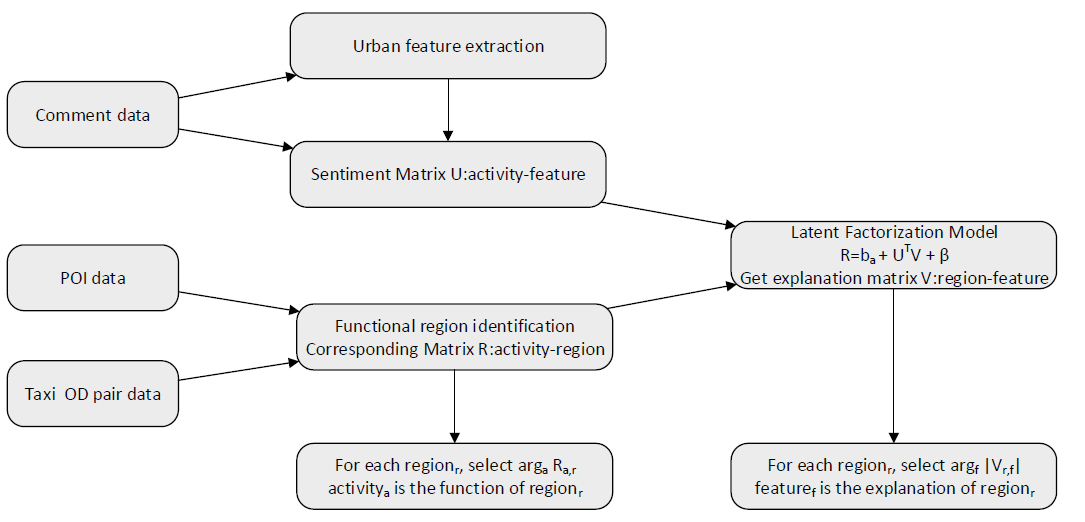
\includegraphics[scale=0.45]{overview.png}
\caption{An illustrative example of Explainable Functional Region Identification (EFRI)}
\label{explanation-example} %% label for entire figure
\end{figure}

%manual label costly supervision in sufficient
The first challenge is how to efficiently extract urban features from online review data.
A naive approach is to maintain a manually constructed lexicon of urban features.
However, the lexicon is expensive to construct and maintain.
An alternative approach is to classify textual phrases with the supervision of a labelled set.
Again, the supervision is costly to obtain.

%unsupervised
To address the first challenge, we adopt an unsupervised approach to extract urban features from online review data.
Urban features are characterized with geographical attributes, existing product feature extraction methods such as~\cite{Lu2011Label} are not directly applicable.
Therefore, we first adopt NLP techniques to select a candidate set of features.
Then we filter urban features which are most representative in geographical texts.

%how to embed mobility data
The second challenge arises from the integration of textual and mobility data.
To fully explain the functional of a region, our goal is to simultaneously discover semantic associations (i.e. how the given region is associated to each urban activity and urban feature) and mobility patterns (i.e. how the current traffic flow of a given region is affected by previous traffic flow).
This is not a trivial task.
The mobility patterns can be highly diverse for each activity and time sensitive.
For example, people tend to gather in school region in the day, while in residence regions produces they gather at night.
Restraining a global form shared by all mobility patterns is problematic.

%bias curve
To address the second challenge, we adopt a layered regression model to embed the semantic associations to predict traffic flows, i.e. the traffic flow of a region is aggregated over all activities, where each activity specific traffic flow is predicted by people's preferences on multiple urban features and the region's association with the same set of urban features.
Furthermore, we incorporate a bias curve in the prediction formula to represent mobility patterns.
The bias curve is free shaped so that the forms of mobility patterns are not restrained.

%contribution
Contribution of this work is three-fold. (1) \textbf{An Unexplored Problem.} To the best of our knowledge, we are the first to study the problem of explainable functional region identification. (2) \textbf{A New Form of Explanations.} We propose a novel framework to deliver explanations. The proposed EFRI explains the functional of a region by demonstrating both the semantics of functional (through urban activities and urban features) and mobility patterns of the functional (time sensitive mobility patterns). Such informative explanations can greatly improve user experience and might shed some insights in other domains such as explainable recommendations. (3) \textbf{A Novel Model.} We present a unsupervised framework to extract urban activities and urban features from online review data. We then adopt a layered regression model to semantically associate regions to urban features. We also embed a free-form bias curve to represent mobility pattrerns in mobility data.

The remainder of the paper is organized as follows.
We briefly overview related work in Section~\ref{sec:related}.
The EFRI system is presented in Section~\ref{sec:extraction} and Section~\ref{sec:regression}.
In Section~\ref{sec:extraction}, we describe technical details to extract urban activities and urban features in online review data.
In Section~\ref{sec:regression}, we give the intuition and inference of the layered regression model to generate explanations that cover both semantic associations and mobility patterns.
We evaluate the EFRI system and analyze the experimental results in Section~\ref{sec:experiments}.
Finally, we conclude this work in Section~\ref{sec:conclusions}.

\section{Related Work}\label{sec:related}
As our work makes use of taxicab pick-ups and drop-offs data and online review data, two lines of work are related: urban computing on mobility data and online review analysis .

%related work section name, find another suitable name for mobility mining
\subsection{Urban Computing on Mobility Data}
%data source
Urban computing~\cite{Zheng2014UrbanConcepts} tackles issues that cities face by analyzing human mobility data.
Major sources of mobility data are check-ins data~\cite{Cheng2011Check-in,Gallegos16happier}, origin-destination pairs data~\cite{Ge2011TaxiBusiness,Meng2017Traffic}  and trajectory data~\cite{Ge2011TaxiBusiness,Garg2018Route,Wu2017Reachable,Wang2018Deep}.The simplest form among them are check-ins data, which is a set of points revealing users' current locations collected from location sharing services. Check-ins data are previously adopted for revealing demographic associations~\cite{Gallegos16happier} and POI recommendation~\cite{Cheng2011Check-in,Zhao2016POI}. Origin-destination data consists of a set of pairwise location points, e.g. a pick-up point and a drop-off point of a taxi trajectory~\cite{Yuan2010NextPassenger,Zheng2011taxicabs}. Most functional region identification systems are based on origin-destination pairs~\cite{Karlsson2006FunctionalRegionSummary}, e.g. from commute data~\cite{Farmer2009Overvie, Korpan2017navigation,Jose2018cognitive}, or from remote-sensor image data~\cite{Vatsavai2011Remote}. Trajectory data consists of a set of routes, where each route is a sequence of location points. Taxi driver trajectory~\cite{Ge2011TaxiBusiness,Garg2018Route} data is more suitable for traffic planning.

%functional region identification
A major and ongoing thrust of research on urban computing concerns the identification of functional regions. In early work, a functional region was defined as a geographical region where the majority of local population recruit and are employed within the region \cite{Ball1980Definition}. Recent studies focus on city-level FRI, i.e. identification of regions in a city that support certain needs of urban lives ~\cite{Yuan2018FunctionRegion}. Traditional FRI systems are rule-based~\cite{Ball1980Definition}, i.e. a city's labor market statistics satisfying certain requirements is considered to be a functional region. Due to the availability of large-scale mobility data, an increasing amount of data-driven approaches~\cite{Farmer2009Overview} have been proposed.
Most of them use clustering methods~\cite{Karlsson2006FunctionalRegionSummary}. To name a few, clustering algorithm based on the 'modularity function'~\cite{Newman2004ModularityFunction,Ratti2010Telecom}, spectral clustering~\cite{Vatsavai2011Remote}, Latent Dirichlet Allocation (LDA)~\cite{Vatsavai2010Remote} and Dirichlet Multinomial Regression (DMR)~\cite{Yuan2018FunctionRegion}.

%drawbacks
Existing urban computing systems extensively rely on complex machine learning algorithms hence they act as blank-boxes for end users.
The lack of explanation weakens the persuasiveness and trustworthiness of the system for end-users.
Our work is to make up for this drawback by providing intuitive explanations of the results for end-users and system designers

\subsection{Online Review Analysis}
Online review data has been extensively studied in opinion mining~\cite{Zhang2018Survey}. Given a set of product features, the user sentiments in each review are extracted either as binary sentiment polarity~\cite{Zhang2015Sentires} or as numerical sentimental strength~\cite{Stieglitz2013SentimentStrenth}. Opinion mining has been combined with recommender systems to generate explainable recommendations~\cite{Zhang2014ExplicitFactor}. Typically, a latent factor model~\cite{Zhang2014ExplicitFactor} is utilized to decompose user-item ratings to a latent feature space of user preferences and item attributes. Though there are fruitful research results in this domain, due to the lack of geographical analysis, these methods are not directly applicable to generate explanations for FRI.

Recently, an emerging research interest is witnessed in exploring the geographical factors that affect online sentiment.
Empirical studies have been conducted on large-scale human mobility data, such as check-in ~\cite{Gallegos16happier}and trajectory~\cite{Gonzlez2008Track},to find the geographical content analysis with sentiment.
Associations are found between online sentiments and geographical factors, e.g happy regions are more likely to connect with each other~\cite{Alshamsi15milan},a high check-in density region usually presents a more positive mode~\cite{Gallegos16happier}, the whole process and development of a organized movement could be tracked on the social media~\cite{Alvarez2015Movement} and so on.

However, most existing work of this line employ simple statistical analysis to uncover the associations.
Such a coarse-grained analysis is distorted by latent variables, such as activity of the region.
Our work is the first to incorporate activity to obtain a fine-grained analysis.


\section{Urban Opinion Extraction}\label{sec:extraction}
%system overview
As shown in Fig.~\ref{explanation-example}, to generate the explanations, the proposed EFRI system consists of two components: (1) \textbf{Urban Opinion Extraction} module works with textual data, such as online POI review data. To be specific, this module first extracts a set of textual phrases that represent urban activities and group the online review data based on activities, then it extracts a set of urban features in each review, finally it extracts the public sentiments on each urban feature under each activity. (2)\textbf{Layered Regression} module works with the results from \textbf{Urban Opinion Extraction} module and mobility data, such as taxicab pick-up and drop-offs data. This module will be discussed in later sections.

\subsection{Urban Activity Extraction}\label{sec:urbanactivityextraction}
%technical details for extracting textual phrases
To obtain a high-quality seed list of phrases , we start with a taxonomy of urban activities.
The taxonomy comes from the self-tags that taken by commented items.
They are given 16 different types of tags, and most of them are consumption.
They form 16 activity sample in the taxonomy, including Residence, Clothing, Study and Scenery and so on.
The taxonomy is easy to obtain and can be used for more activities.

%is it too many or too few? If it's too many, use the seed list as a supervision set. If it's too few, describe the filtering method below.
However, the seed list is too few to describe various functions.
Intuitively, a good activity phrase should have the ability to find the major function of at least a label.
The quantity of few activity constrains the activities hidden in textual data.
Therefore, we applied a k-Nearest Neighbor(KNN) to find more activity phrases based on the 16 activity samples mentioned in last step.
We select all words whose property is noun and sort them into vectors with word embedding.
By measure the consine distance between two vectors that stands for two words, we can find the k closest neighbors of each word.
Different with traditional kNN, we aim to find suitable activity features instead of classification.
A word can be select as activity if the score of positive examples, i.e. selected activity phrases, in its k neighbor are larger than a threshold.
There is very few positive examples in the beginning, so we give the 16 original activity a large weight.
Meanwhile, the confidence of later positive examples is set by their neighbors.
A word with many positive example neighbors and high-weight neighbors would get high weight.
The process consists until no new activity is found.

%group textual data based on activity
We obtain a set of activity phrases $\mathcal{A}=\{a\}$ after the above two steps.
We group the textual data based on the recognized activity phrases.
A sentence include a activity means it is contains relative information about the activity.
We can classify it into the responding activity.
Specially, a sentence may include several activities, which could be analysed in different activities without conflict.

\subsection{Urban Feature Extraction}\label{sec:urbanfeatureextraction}
%features
Previous studies on opinion mining for product recommendations~\cite{Zhang2014ExplicitFactor} have achieved remarkable success in extracting product aspects, i.e. with a precision more than $90\%$.
In our EFRI models, the features would be displayed as explanation for the labels, which relate the activities with labels.
A high similarity between activities and urban features would help improve the persuasiveness of our explanation.
In next step, we will find sentiment correlate with urban features in grouped textual data of activity.
Similarity between activity and features also provide more analytical corpus.
Therefore, we choose word2vec~\cite{Mikolov2013Word2vec} to find the most relative words between selected activities.
Word2vec is superior than consine distance in terms of similarity of semantics, for it is based on complex neural network.
A feature semantically similar to activity make user easier to associate the feature with possible activities.
Feature is a word with a similarity accumulation with each activity phrase large than a threshold.
Frequency from statistic is also an important criteria here.
As we are building a candidate list, the primal objective is to obtain high coverage instead of high precision.

%filter features
\emph{Urban features} distinguish with product aspect in that it denotes geographical characters of different functional region.
Intuitively, a phrase indicating an urban feature must be relative to special characters as well as make distinguishment in regions with different labels
As forth, we use information gain(IG) to selected our urban features as:

\begin{align*}
IG(word) =& H(C)-H(C|W)\\
=&-\sum_{i=1}^{k}P(C_i)\log_2P(C_i)+P(word)\sum_{i=1}^{k}P(C_i|word)\log_2P(C_i|word)\\
&+P(\overline{word})\sum_{i=1}^{k}P(C_i|\overline{word})\log_2P(C_i|\overline{word})
\end{align*}
where $P(word)$ is the proportion the word while $P(\overline{word}) = 1- P(word)$;
$C_i$ denotes the $i$-th class;
information entropy $H(C)$ reflects the degree of uncertainty of information. The greater the entropy, the more unstable the features are;
conditional entropy $H(C|W)$ demonstrates the degree of uncertainty after classification according to this feature, and a small conditional entropy denotes a more stable case after classification.
A high IG value means the word contributes a lot in such a classification.
and we select features with highest IG value as urban features.

The selected features are shown in Table~\ref{tab:urbanfeatures}

\begin{table}[h]
\centering
\caption{Selected Urban Features}
\label{tab:urbanfeatures}
\begin{tabular}{c|c|c|c|c}
\hline
features &  Alley & Brand & Center & Square\\
\hline
information entropy &  &  &  & \\
\hline
\end{tabular}
\end{table}


\subsection{Urban Sentiment Extraction}
%sentiment
We do not focus on word-level sentiment analysis in this paper.
The common used approach to get sentiment score is based on lexicon.
We rate the sentiment score of textual data with a existed lexicon with.
Each word in the lexicon has a trained rate of sentiment.
With the sopport of stopwords, negative words and adverbs with degree, we could get the sentiment rating of whole sentence.

%aggregate sentiments
However, the problem of aggregating word-level sentiments to activity must be addressed.
In the Section~\ref{sec:urbanactivityextraction}, we have group textual data with different activities.
And in the Section~\ref{sec:urbanfeatureextraction}, we extract urban feature by similarity with activities.
Due to the similarity we could find enough relevant textual data between each pair of activities and urban features.
For each activity $a$, we search each urban feature in its corresponding textual data.
If a sentence in textual data of $a$ contains urban feature $k$, we calculate its sentiment score as a candidate value of $U_{a,k}$.
The final value of $U_{a,c}$ is the average value of its candidates.
To fit the sentiment polarity, we map each value of $U_{a,c}$ into the range of $[-1,1]$ by a variant of $sigmoid$ function as:
$$f(x) =\frac{2}{1+\exp(-x)}-1$$
Now we get a matrix $U$, which denotes the sentiment on corresponding activities and urban features.

\section{Layered Regression Model}\label{sec:regression}
%preliminaries
In this section, we describe in detail the layered regression model. Hereafter, unless stated otherwise, we use lower-case letters for indices, uppercase letters for sets, lower-case bold-face letters for vectors and upper-case bold-face letters for matrices. To be specific, an arbitrary FRI system divides a city into a set of regions, denoted as $r\in R$ and each region $r$ is labeled by $l\in L$. From textual data, the urban opinion extraction module obtains public sentiment $\mathbf{U}_a\in \mathcal{R}^{K}$ on each activity $a\in A$, where $\mathbf{U}_{a,k}$ is the public sentiment on urban feature $k$ under activity $a$. The mobility data consists of number of visitors $f_{r,t}$ for each region $r\in R$ at each time-point $t=1,\cdots,T$. $f_{r,t}$ can only be non-negative. More notations are shown in Table~\ref{tab:notation}

\begin{table}[htp]
\caption{Notations for layered regression model}
\begin{center}
\begin{tabular}{|c|c|}
\hline
Notation & Description \\\hline
${A}=\{a\}$ & a set of activities \\
${R}=\{r\}$ & a set of regions \\
${L}=\{l\}$ & a set of labels \\
$F=\{f_{r,l,t}|f_{r,l,t}\geq 0\}$ & A set of observed number of visitors for region $r$ with label $l$ at time $t$ \\
$\mathbf{U}_a\in \mathcal{R}^K$ & Extracted public sentiments on each urban feature under activity $a$ \\
$\mathbf{V}_r\in \mathcal{R}^K$ & Parameter representing the relevance of each urban feature to region $r$\\
$\mathbf{c}_{l}\in \mathcal{R}^{|A|}$ & Coefficient of label $l$ to each activity\\
$b_t$ &  Traffic flow bias at time $t$\\
\hline
\end{tabular}
\end{center}
\label{tab:notation}
\end{table}%

\subsection{Traffic Flow Prediction}
Our model builds on a simple intuition, that the more people will visit a region $r$ to perform an activity $a$, if the region $r$ is more relevant to the desired urban features under the activity $a$.
The desired urban features under activity $a$ is encoded in $\mathbf{U}_a$ which is extracted from online review data.
The relevance of region $r$ to each urban feature is encoded in $\mathbf{V}_r$ which needs to be learnt.
Therefore, the number of visitors $\hat{f}_{r,a}$ can be predicted as follows:
\begin{equation}\label{equ:fra}
\hat{f}_{r,a}= \mathbf{U}_a^T \mathbf{V}_r
\end{equation}

Clearly, people visit a place to perform various activities.
Thus for a region $r$ at time $t$, the traffic flow is aggregated over all possible activities. This leads to the following equation:
\begin{equation}
\hat{f}_{r,l,t}=b_t+\sum_{a} \mathbf{c}_{l,a} [\mathbf{U}_a^T V_r+  \beta_{a,t} (f_{r,l,t-1})] \label{equ:model}
\end{equation}
where in the left $\hat{f}_{r,l,t}$ is the observed traffic flow at time $t$ for region $r$ that has been labeled $l$ in the mobility data. In the right, the first term $b_t$ is a bias term, the second term considers how much traffic flow each activity brings to a region $r$ with label $l$, $\mathbf{c}_{l,a}$ measures coefficients between label $l$ and activity $a$. $\mathbf{c}_{l}>\mathbf{0}$. It is worthy to note here that $\mathbf{c}_l$ must be learnt across all regions associated with label $l$. In this manner, the semantics of label $l$ by the FRI can be interpreted through the activities (the name ``layered'' regression comes from the layered framework of activity and label).

We usually observe mobility patterns for traffic flows.
These patterns can be highly diverse across activities.
For example, school regions (high traffic flow in the day) and business regions (high traffic flow at night) have different mobility patterns.
Also it is reasonable to assume temporal dependency in traffic flows.
Again the temporal dependencies vary among activities.
For example, current number of visitors in business regions might be strongly influenced by previous numbers of visitors, while in school regions the influence is not significant.

Such diverse and dynamic mobility patterns are modeled by the bias curve $\beta_{a,t}(f_{r,l,t-1})$.
The subscript $a$ suggests that the bias curve is activity specific.
The subscript $t$ suggests that the bias curve is time sensitive, i.e. with different forms at night and in the day. To reduce the number of model parameters, we can group $t$ to a limited set of time segments. For example, if we consider only ``weekends'', ``weekday day''  and ``weekday night" then there are in total $3\times |A|$ bias curves.

To capture the diverse nature of bias curve, the form of $\beta(x)$ is unknown.
We apply a data-driven approach: kernel regression, which is a typical non-parameter learning method to fit $\beta(x)$.

\begin{equation}\label{eqn:kernel}
\beta_{a,t} (x) = \frac{\sum_{i=1}^n k_h(x-x_i) y_i}{ \sum_{j=1}^n k_h(x-x_j)}
\end{equation}

To obtain the set of samples $\{(x_i,y_i)\},i=1,\cdots,n$, we let $x_i$ to be uniformly sampled from the range of $f_{r,l,t-1}$. $k_h(x-x_i)= \exp(-h (x-x_i)^2)$, where $h$ is a hyper-parameter to control the smoothness of the function. The set of $y_i$ are to be learnt from data.

\subsection{Model Inference}
Finally, we set up the objective function for layered regression model.
\begin{eqnarray}
\min \mathcal{L} & =\sum_{f_{r,l,t}\in F}(f_{r,l,t}-\hat{f}_{r,l,t})^2+\lambda_1 (\sum_t b_t^2  + \sum_r \|\mathbf{V}_r\|^2 )\\\nonumber
& +\lambda_2(\sum_l \|\mathbf{c}_l\|_1)+\lambda_3(\sum_i y_i^2)\\\nonumber
& w.r.t. \forall l, \mathbf{c}_l\geq \mathbf{0}
\label{equ:loss}
\end{eqnarray}

The first term in Equ.~\ref{equ:loss} minimizes the differences between observed traffic flow and predicted traffic flow by Equ.~\ref{equ:model}. The second term avoids over-fitting by adding a L2 penalty term on model parameters $b_t, \mathbf{V}_r$. The third term further regularizes the squared loss by adopting a L1 term on $\mathbf{c}_l$. The sparseness constraint on $\mathbf{c}_l$ helps to represent a label by the most representative activity.

The parameters are inferred by stochastic gradient.

\begin{align*}
b_t &= b_t - \gamma\left(-2\times\left(\sum_{l,r}(f_{r,l,t} - \hat{f}_{r,l,t})\right)+2\times\lambda_1\times b_t\right)\\
V_{f,r} &= V_{f,r} - \gamma\left(-2\times\left(\sum_{l,r}(f_{r,l,t} - \hat{f}_{r,l,t})\times\left(\sum_ac_{l,a}\times U_{a,f}\right)\right)+2\times\lambda_1\times V_{f,r}\right)\\
c_{l,a} &= c_{l,a} - \gamma\left(-2\times(\sum_{l,r}(f_{r,l,t} - \hat{f}_{r,l,t})\times(U_a^TV_r + \beta_{a,t}(\hat{f}_{r,l,t-1})))+\lambda_2\right)\\
y_i &= y_i - \gamma\left(-2\times\left(\sum_{l,r}(f_{r,l,t} - \hat{f}_{r,l,t})\times\left(\sum_a c_{l,a}\frac{k_h(\hat{f}_{r,l,t-1}-x_j)}{\sum_{j=1}^n k_h(\hat{f}_{r,l,t-1}-x_j)   }\right)\right)+2\times\lambda_3\times y_i\right)\\
\label{equ:sgd}
\end{align*}
where $\gamma$ is the learning rate.

\section{Experiments}\label{sec:experiments}
In this section we ask the following research questions.
(1) Does the proposed EFRI framework accurately extract urban features?
(2) Does EFRI capture the mobility patterns?
(3) Does EFRI improve the interpretability of FRI results?

\subsection{Experimental Setup}
The data sets for our experiments include a mobility data set and a textual data set.
The mobility data (Didi dataset) is a set of  pick-up and drop-off coordinates of taxicabs with timestamps.
It contains more than 7 million pick-up and drop-off pairs in November 2016.
The textual data set (Dianping dataset) is a set of comments of various items.
It is crawled from China's largest online review sites\footnote{www.dianping.com.cn} Before August 2018.
We search for all corresponding items with 16 tags located within five center districts in the city respectively.
Most introduction page of each item also provides the coordinate and comments of it.
The data set contains 109686 POIs and 3213264 comments.


\subsection{Pre-processing}

%preprocessing
To obtain the input for EFRI, we implement four pre-processing steps: (1) region segmentation; (2) data set linking; (3)FRI on mobility data; (4) text cleaning.

\textbf{Region segmentation.} To form the basic city regions, we segment the urban area by the city's major road network.
The longitude of the map range in Didi dataset is [103.93,104.21] and latitude range is [30.56,30.79], which covers the main area of a city.
Most of the POIs also located within the area.
We downloaded the major road network of this region\footnote{http://www.bigemap.com/} and rasterized the area into a 2000 $\times$ 2400 grid by ArcMap, a professional map processing software.
The road network is converted to a grey image, where in each grid 1 stands for the road and $0$ otherwise.
The dilation and thinning process~\cite{Yuan2018FunctionRegion} is operated to remove small regions such as lanes and road overpasses and simplify the map.

\textbf{Data set linking.} The common ground of the two datasets is that they both have specific coordinates, which could be corresponding to the rasterized grid exactly.
For mobility data, we find the traffic flow of each region, and list the flow as vector by time.
And for POI data, we list the interests of POIs of each region as vector, and the dimension of this vector is equal to the quantity of POIs.
Now each region has two vectors, and they are the input of DMR.

\textbf{FRI on mobility data.} We use DMR~\cite{Yuan2018FunctionRegion} to identify region functionals and label them with 8 types.
DMR is operate with hyper-parameters $\beta = 0.01$, variance $\sigma^2 = 1$
Note that we can use any convenient FRI system to identify region functionals.
The DMR results are illustrated in Figure~\ref{fig:DMR}


\begin{figure}[h]
\centering
\subfigure[After dilation operator]{
\label{thin_result} %% label for second subfigure
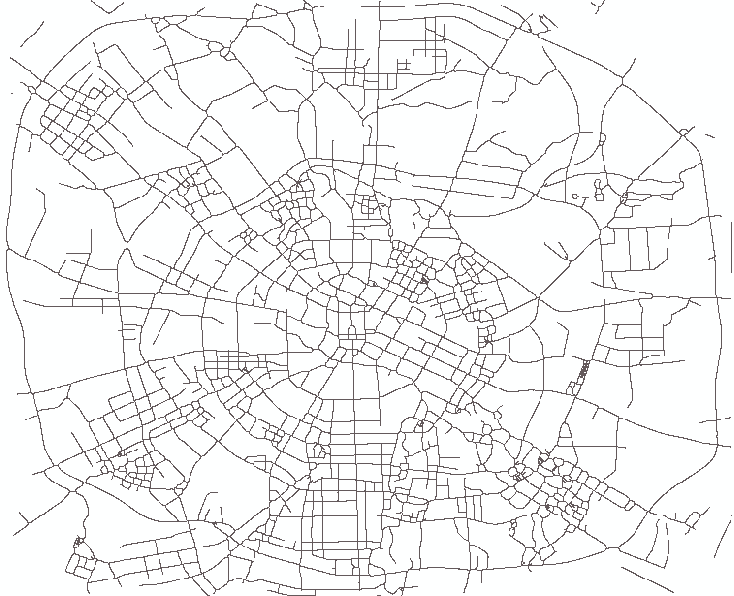
\includegraphics[width=2.3in]{FunctionalRegions_thinning.png}}
\subfigure[segmented region units of the city]{
\label{DMR_result} %% label for second subfigure
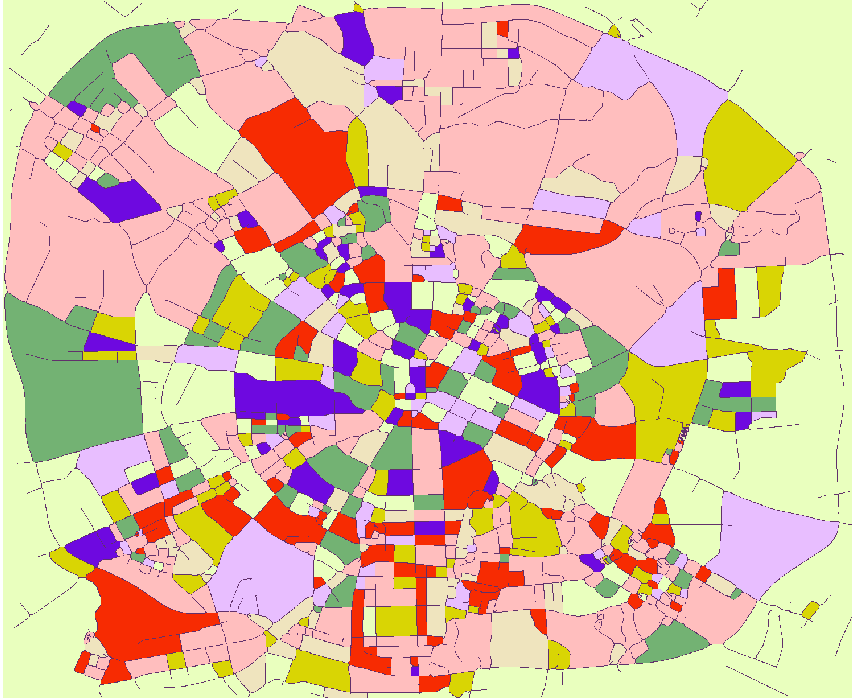
\includegraphics[width=2.3in]{FunctionalRegions_DMR.png}}
\caption{results of DMR}
\label{fig:DMR}
\end{figure}



\textbf{Text Cleaning.}
A common used package for Chinese word segmentation is Jieba Segment Word.
We use it to deal with raw textual data and
We gather 883 words with less information as stopwords.
To save memory and improve efficiency, the stopwords are removed from the segmented word list and don't continue the following analysis.
%activity extraction?  Sec3.1 has done.
Statistics of the combined dataset are shown in Table~\ref{tab:dataset}.
Averagely, a POI is associated with nearly 30 comments, a region is related to over 15000 mobility trajectories in 30 days,
 and a label contains over 100 regions.

\begin{table}[h]
\centering
\caption{Statistics of dataset}\label{tab:dataset}
\begin{tabular}{|c|c|c|c|c|}
\hline
\#POIs & \#Comments & \#Mobility pairs & \#Regions & \#Labels \\
\hline
109686 & 3213264 & 7065937 & 901 & 8 \\
\hline
\end{tabular}
\end{table}

\subsection{Urban Feature Extraction}
We aim to select suitable urban feature which has a strong distinction on various region functions.

\textbf{Comparative Methods.} We compare EFRI with the following systems. (1) Frequency; (2)TF-IDF; (3)rule-based.

A simple baseline is to selected the nouns with highest frequency, i.e. appear in as much comments as possible.
The common approach to extract feature is term frequency�Cinverse document frequency(TF-IDF) as:
$$TF-IDF(x) = TF(x)\times IDF(x) = (\log\frac{N}{N(x)})\times(\log\frac{N(x)}{N(x)+1}+1)$$
where $N$ is the quantity of whole text data ,and $N(x)$ is the quantity of text data contain word $x$
%Introduction of rule-based.I haven't find related tutorial

\textbf{Evaluation metrics.} These metrics are used to measure our performance:
(1)Normalization Discounted Cumulative Gain(NDCG); (2)p@n.

To evaluate the accuracy of urban feature extraction, five human volunteers are required to give every selected feature a rating $gain$ of ranges from 1 to 5.
NDCG is a common used measure, which incorporates graded relevance. The form is:
\begin{align*}
DCG_p&=\sum_{i=1}^{p}\frac{gain_i}{\log_2(i+1)}\\
DCG_p&=\sum_{i=1}^{|REL|}\frac{gain_i}{\log_2(i+1)}\\
NDCG_p&= \frac{DCG}{IDCG}
\end{align*}
NDCG@$k$ means that $k$ features are selected to be evaluated.
And p@n represents the proportion of features with cumulative Gain higher than 2 in n selected urban features.

\begin{table}[h]
\centering
\caption{Comparative performance of urban feature extraction}\label{tab:extraction}
\begin{tabular}{p{3.3cm}|p{1.6cm}|p{1.6cm}|p{1.6cm}|p{1.6cm}|p{1.6cm}}
        \hline
        Extraction approach & p@5 & p@10 & p@15 & NDCG@3 & NDCG@5\\
        \hline
        Frequency &  &  &  & \\
        \hline
        TF-IDF &  &  &  & \\
        \hline
        rule-based &  &  &  & \\
        \hline
        EFRI &  &  &  & \\
        \hline
    \end{tabular}
\end{table}

As shown in Table~\ref{tab:extraction}, We can see that our EFRI model has a superior performance of urban feature extraction.

\subsection{Traffic Flow Prediction}

\textbf{Comparative Methods.} The prediction of EFRI is operated with layered regression.
There is some other approaches can estimate the prediction. (1)collaborative filtering; (2)EFRI withour bias curve $\beta$; (3) EFRI with normal feature.

CF is widely used in recommendation system.Therefore, prediction is one of the most application of CF.
Meanwhile, we compare with the variant form of EFRI to validate its advantage.

\textbf{Evaluation metrics.}It is a typical regression process and common used evaluate matrix is: (1)Mean Squared Error(MSE), (2)Root Mean Squared Error(RMSE), (3)Mean Absolute Error(MAE) (4)R Squared($R^2$).

They are typical metrics to measure the accuracy of regression model, and their form as:
$$MSE = \frac{1}{m}(y_i-\hat{y}_i)^2$$
$$RMSE = \sqrt{\frac{1}{m}(y_i-\hat{y}_i)^2}$$
$$MAE = \frac{1}{m}|y_i-\hat{y}_i|$$
$$R^2 = 1-\frac{MSE(\hat{y} , y)}{Var(y)}$$
where $y$ is the real value and $\hat{y}$ is the predict value given by regression;
$Var(y)$ is the variance of $y$.

\begin{table}[h]
    \centering
    \caption{Comparative performance of traffic flow prediction}\label{tab:prediction}
    \begin{tabular}{p{3.3cm}|p{1.6cm}|p{1.6cm}|p{1.6cm}|p{1.6cm}}%{c|c|c|c|c|c}
        \hline
        Prediction Approach & MSE & RMSE & MAE & $R^2$ \\
        \hline
        CF &  &  &  & \\
        \hline
        EFRI without $\beta$ &  &  &  & \\
        \hline
        EFRI with normal feature &  &  &  & \\
        \hline
        EFRI &  &  &  & \\
        \hline
    \end{tabular}
\end{table}
From Table~\ref{tab:prediction}, we confirm our confidence that EFRI has a more accurate result than other approaches in most metrics.
It turn out that EFRI could capture the interesting information in mobility patterns.
EFRI perform better than the same framework with normal feature, which also proves the accuracy of our urban feature extraction.

Besides, the variable $y_i$ corresponding to $x_i$ have been learn by EFRI, and we get parameter of $\beta(x)$.
The form of $\beta(x)$ with trained $y_i$ is shown in Figure~\ref{fig:beta}
\begin{figure}[h]
  \centering
  \label{fig:beta}
  \caption{The form of $\beta$ with a=1, t=weekend}
\end{figure}


\subsection{Explainability Performance}

\textbf{Comparative Methods.} We compare EFRI with the following systems. (1)text-based explanation; (2)trajectory-based explanation.

EFRI based on the mixture application of mobility data and textual data.
We set the explanation given by a single data source as baseline to discuss the result of the heterogeneous data.

\textbf{Evaluation metrics.} Evaluation of explainable systems is still an open problem. In this work, we consider two categories of evaluation metrics. The first is objective to evaluate the quantity of explanations. (1)explainability precision(EP); (2)Explain quality.

To measure the explainability of these models, ~\cite{Abdollahi2017MEPMER} adopted MAP and MAR as evaluation metrics.
EP is percentage of regions that could find explanation label by our framework, which is defined as:
$$explanation\ percentage=\frac{|regions\ with\ explanation\ label|}{|all\ regions|}$$
And the rest are subjective to evaluate the quality of explanations.

All reported results are averaged over regions.

\textbf{Evaluation Process}
To measure the quality of explainability, five human volunteers are required to give every urban feature as explanation a rating.
The accurate labels get 5 stars while the incorrect get 1 star.
Our evaluation based on the average of the rating over humans.

\begin{table}[h]
\centering
\caption{Comparative performance of explainability }\label{tab:explainablity}
\begin{tabular}{p{3.3cm}|p{2.2cm}|p{2.2cm}|p{2.2cm}|p{2.2cm}}
        \hline
        Method & EP & Explain quality\\
        \hline
        text-based &  & \\
        \hline
        Trajectory-besed &  & \\
        \hline
        EFRI &  & \\
        \hline
    \end{tabular}
\end{table}

As shown in Table~\ref{tab:explainablity}, EFRI is outperformed than the baselines with single data source in both EP and quality.
It demonstrates that our mixture of the heterogeneous data improve the interpretability of FRI results.




\subsection{Case Study}
Finally we demonstrate a case study. As shown Figure~\ref{fig:DMR}, regions in the city can be roughly classified as residence region, business region, study and science region and scenery regions.
\begin{table}[h]
\centering
\caption{Functional Regions and corresponding urban feature}\label{dataset}
\begin{tabular}{c|c}
\hline
Functions & Urban Feature\\
\hline
Business & \\
\hline
Residence & \\
\hline
Study & \\
\hline
Scenery & \\
\hline
\end{tabular}
\end{table}






\section{Conclusion}\label{sec:conclusions}
We present a novel explainable functional region identification (EFRI) system.
We provide post-hoc explanations which describe the results of any FRI system through a set of urban activities and urban features automatically extracted from online textual data.
We further embed the diverse and time-sensitive mobility patterns revealed in mobility data with semantic associations in textual data.
Experiments show that our system can extracted high quality urban features and provide reasonable explanations.

In future work we will explore more information sources such as tweets and news reports to incorporate the power of big data in EFRI.
With massive amounts of textual data that covers all areas of urban lives, more human activities can be explained.
Another future direction is to adopt new styles of explanations.
For example, explanations in nature language are more friendly to end-users.
Visualizing the explanations is beneficial for government officers and system designers.


\begin{thebibliography}{25}
\bibitem{Zheng2014UrbanConcepts}Zheng Y, Capra L, Wolfson O, et al. Urban Computing:Concepts, Methodologies, and Applications[J]. Acm Transactions on Intelligent Systems \& Technology, 2014, 5(3):1-55.
\bibitem{Yuan2018FunctionRegion}Yuan N J, Zheng Y, Xie X. Discovering Functional Zones in a City Using Human Movements and Points of Interest[J]. 2018.
\bibitem{Karlsson2006FunctionalRegionSummary}Karlsson C, Olsson M. The identification of functional regions: theory, methods, and applications[J]. Annals of Regional Science, 2006, 40(1):1-18.
\bibitem{Newman2004ModularityFunction}Newman M E J. Detecting community structure in networks[J]. European Physical Journal B, 2004, 38(2):321-330.
\bibitem{Ratti2010Telecom}Ratti C, Sobolevsky S, Calabrese F, et al. Redrawing the Map of Great Britain from a Network of Human Interactions[J]. Plos One, 2010, 5(12):e14248.
\bibitem{Vatsavai2011Remote}Vatsavai R R, Bright E, Varun C, et al. Machine learning approaches for high-resolution urban land cover classification:a comparative study[C]// International Conference and Exhibition on Computing for Geospatial Research \& Application, Com.geo 2011, Washington, Dc, Usa, May. DBLP, 2011:1-10.
\bibitem{Vatsavai2010Remote}Vatsavai R R, Cheriyadat A, Gleason S. Unsupervised Semantic Labeling Framework for Identification of Complex Facilities in High-Resolution Remote Sensing Images[C]// IEEE International Conference on Data Mining Workshops. IEEE Computer Society, 2010:273-280.
\bibitem{Preece2018ExplainAI}Preece A. Asking 'Why' inAI: Explainability of intelligent systems - perspectivesand challenges. Intell Sys Acc Fin Mgmt. 2018;25:63-72.
\bibitem{Korpan2017navigation}Korpan, R., Epstein, S.L., Aroor, A., Dekel, G.: WHY: Natural explanations from a robot navigator. In: AAAI 2017 Fall Symposium on Natural Communication for Human-Robot Collaboration.
\bibitem{Jose2018cognitive}Jose M. Alonso, Corrado Mencar. Building Cognitive Cities with Explainable Artificial Intelligent Systems. In Proceedings of the First International Workshop on Comprehensibility and Explanation in AI \& ML, 2017.
\bibitem{Lu2011Label}Lu Y, Castellanos M, Dayal U, et al. Automatic construction of a context-aware sentiment lexicon:an optimization approach[C]// International Conference on World Wide Web, WWW 2011, Hyderabad, India, March 28 - April. DBLP, 2011:347-356.
\bibitem{Cheng2011Check-in}Z. Cheng, J. Caverlee, K. Lee, and D. Sui. Exploring millions of footprints in location sharing services. In International AAAI Conference on Web and Social Media, 2011.
\bibitem{Gallegos16happier}Gallegos L, Huang A, Huang A, et al. Geography of Emotion: Where in a City are People Happier?[C]// International Conference Companion on World Wide Web. International World Wide Web Conferences Steering Committee, 2016:569-574.
\bibitem{Ge2011TaxiBusiness}Ge Y, Liu C, Xiong H, et al. A taxi business intelligence system[C]// ACM SIGKDD International Conference on Knowledge Discovery and Data Mining, San Diego, Ca, Usa, August. DBLP, 2011:735-738.
\bibitem{Meng2017Traffic}Meng, C.; Yi, X.; Su, L.; Gao, J.; Zheng, Y. City-wide Traffic Volume Inference with Loop Detector Data and Taxi Trajectories. Proceedings of the 25th ACM SIGSPATIAL International Conference on Advances in Geographic Information Systems,ACM,2017, 1:1-1:10
\bibitem{Garg2018Route}Nandani Garg and Sayan Ranu. Route Recommendations for Idle Taxi Drivers: Find Me the Shortest Route to a Customer!. In KDD 18: The 24th ACM SIGKDD International Conference on Knowledge Discovery \& Data Mining, August 19-23, 2018, London, United Kingdom. 2018.
\bibitem{Wu2017Reachable}Wu G, Ding Y, Li Y, et al. Mining Spatio-Temporal Reachable Regions over Massive Trajectory Data[C]// IEEE, International Conference on Data Engineering. IEEE, 2017:1283-1294.
\bibitem{Wang2018Deep}D Wang,J Zhang,W Cao,J Li,Y Zheng.When Will You Arrive? Estimating Travel Time Based on Deep Neural Networks.In International AAAI Conference on Web and Social Media, 2018.
\bibitem{Zhao2016POI}Zhao S, King I, Lyu M R. A Survey of Point-of-interest Recommendation in Location-based Social Networks[J]. 2016.
\bibitem{Zheng2011taxicabs}Zheng Y, Liu Y, Yuan J, et al. Urban computing with taxicabs[C]// International Conference on Ubiquitous Computing. ACM, 2011:89-98.
\bibitem{Yuan2010NextPassenger}Yuan J, Zheng Y, Zhang L, et al. Where to find my next passenger[C]// Proceedings of the 13th international conference on Ubiquitous computing. ACM, 2011:109-118.
\bibitem{Farmer2009Overview}Farmer, C. J. (2009). Data driven functional regions. In Proceedings of 10th International Conference on GeoComp
\bibitem{Ball1980Definition}R.M. Ball. The use and definition of Travel-to-Work Areas in Great Britain: Some problems[J]. Regional Studies, 1980, 14(2):125-139.
\bibitem{Zhang2018Survey} Zhang Y, Chen X. Explainable Recommendation: A Survey and New Perspectives[J]. arXiv preprint arXiv:1804.11192. 2018.
\bibitem{Zhang2015Sentires}  Zhang Y, Zhang M, Liu Y, et al. Boost Phrase-level Polarity Labelling with Review-level Sentiment Classification[J]. Computer Science, 2015.
\bibitem{Stieglitz2013SentimentStrenth}Stieglitz S , Dang-Xuan L . Emotions and Information Diffusion in Social Media��Sentiment of Microblogs and Sharing Behavior[J]. Journal of Management Information Systems, 2013, 29(4):217-248.
\bibitem{Zhang2014ExplicitFactor}Zhang Y, Lai G, Zhang M, et al. Explicit factor models for explainable recommendation based on phrase-level sentiment analysis[C]// International Acm Sigir Conference on Research \& Development in Information Retrieval. ACM, 2014:83-92.
\bibitem{Gonzlez2008Track}Gonzlez M C, Hidalgo C A. Understanding individual human mobility patterns[J]. Nature, 2008, 453(7196):779-782.
\bibitem{Alshamsi15milan}Alshamsi A, Awad E, Almehrezi M, et al. Misery loves company: happiness and communication in the city[J]. Epj Data Science, 2015, 4(1):7.
\bibitem{Alvarez2015Movement}R. Alvarez, D. Garcia, Y. Moreno, and F. Schweitzer. Sentiment cascades in the 15m movement. EPJ Data Science, 4(1):1-13, 2015
\bibitem{Mikolov2013Word2vec}Mikolov T , Sutskever I , Chen K , et al. Distributed Representations of Words and Phrases and their Compositionality[J]. Advances in Neural Information Processing Systems, 2013, 26:3111-3119.
\bibitem{Abdollahi2017MEPMER}Behnoush Abdollahi and Olfa Nasraoui. Using explainability for constrained matrix factorization. In Proceedings of the Eleventh ACM Conference on Recommender Systems, pages 79�C83. ACM, 2017.



\bibitem{Herlocker2000Explanation} Herlocker J L, Konstan J A, Riedl J. Explaining collaborative filtering recommendations[C]// Acm Conference on Computer Supported Cooperative Work. 2000:241-250.
\bibitem{Ferwerda2012ContentCorrelate} Ferwerda B, Swelsen K, Yang E. Explaining Content-Based Recommendations[J]. Bruceferwerda Com.
\bibitem{Zhang2017Model}Zhang X , Zhao J , Lui J C S . Modeling the Assimilation-Contrast Effects in Online Product Rating Systems: Debiasing and Recommendations[C]// Eleventh Acm Conference on Recommender Systems. ACM, 2017.
\end{thebibliography}
\end{document} 